\documentclass[]{article}

\usepackage[utf8]{inputenc}
\usepackage[paperheight=1.in,paperwidth=2.6in,margin=0in]{geometry}
\usepackage{tikz}
\usetikzlibrary{shapes,arrows,automata,calc}
\usepackage{color}

\usepackage{booktabs}  % nicer table borders 

\begin{document}

%\clearpage
%\thispagestyle{empty}

\tiny{
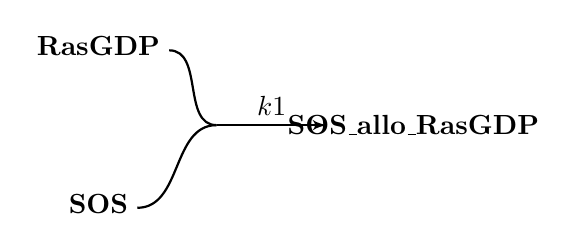
\begin{tikzpicture}[auto, outer sep=0pt, node distance=0cm,>=latex']

\node at (0, 0) (RAS_GDP) {$\bf RasGDP$};
\node at (0, -2) (SOS) {$\bf SOS$};
\node at (4, -1) (ALLO) {$\bf SOS\_allo\_RasGDP$};
\node at (1.5, -1) (MIDPOINT) {};
    \draw [->, thick] ($(MIDPOINT)$) to node {$k1$}
    ($(ALLO)+(-1.1,0)$);
    \path [-, thick] ($(RAS_GDP.east)+(0,-0.05)$) edge[in=180, out=0]
    ($(MIDPOINT)$);
    \path [-, thick] ($(SOS.east)+(0, -0.05)$) edge[in=180, out=0]
    ($(MIDPOINT)$);
\end{tikzpicture} 
}

\end{document}

